\documentclass[landscape]{article}
\usepackage{geometry,tikz}
\usetikzlibrary{trees,calc}
\geometry{paperwidth=30cm, paperheight=10cm,left=2pt,right=2pt,top=2pt,bottom=2pt}
\pagestyle{empty}
\setlength{\parindent}{0pt}
\tikzset{%
model/.style={left,rotate=90},
submodel/.style={rotate=45},
}
\begin{document}
\centering
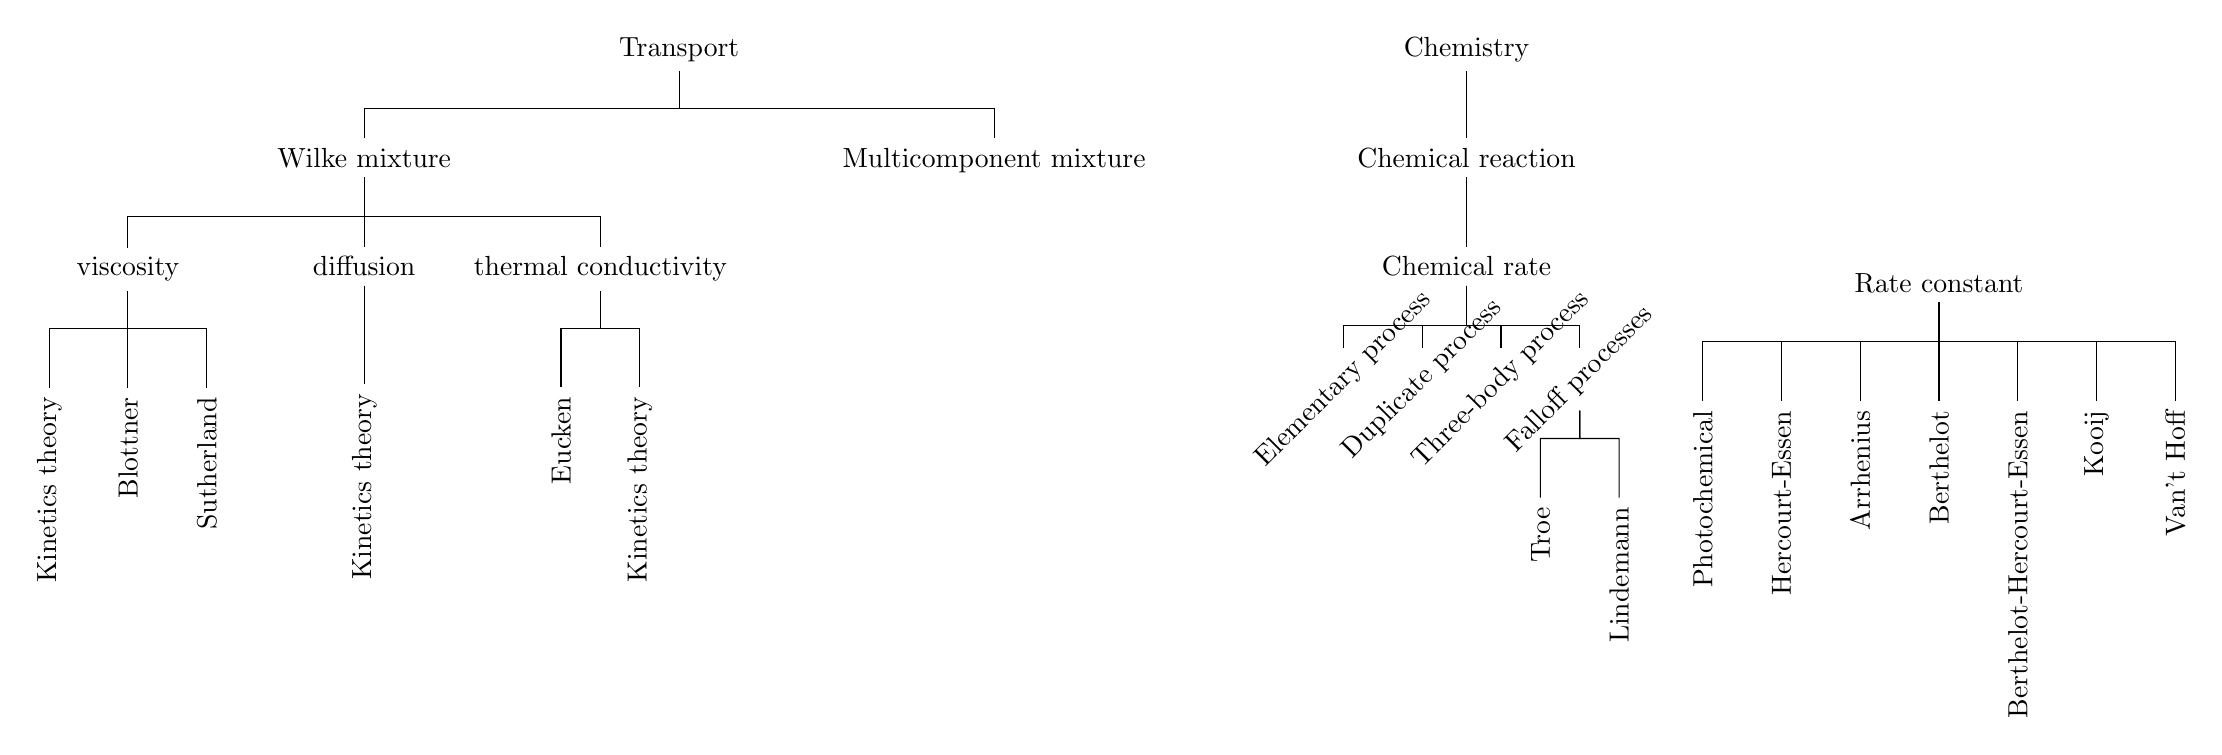
\begin{tikzpicture}[remember picture,
                    every node/.append style={anchor=base},
                    level 1/.style={edge from parent fork down, sibling distance=8cm},
                    level 2/.style={sibling distance = 3cm},
                    level 3/.style={sibling distance = 1cm}]

\node (chimie) at (10,0) {Chemistry} 
            child    
                 { node {Chemical reaction}
                   child { node {Chemical rate}
                      child{ 
                             node[submodel] {Elementary process}
                           }
                      child{ 
                             node[submodel]{Duplicate process}
                           }
                      child{ 
                             node[submodel]{Three-body process}
                           }
                      child{ 
                             node[submodel]{Falloff processes}
                             child {
                                      node[model] {Troe}
                                   }
                             child {
                                      node[model] {Lindemann}
                                   }
                           }
                        }
                 };

\node (rate) at (16,0) {}
                child[draw=white]{ node {}
                 child { node {Rate constant}
                   child[draw=black] { 
                          node[model] {Photochemical}
                        }
                   child[draw=black] { 
                          node[model] {Hercourt-Essen}
                        }
                   child[draw=black] { 
                          node[model] {Arrhenius}
                        }
                   child[draw=black] { 
                          node[model] {Berthelot}
                        }
                   child[draw=black] { 
                          node[model] {Berthelot-Hercourt-Essen}
                        }
                   child[draw=black] { 
                          node[model] {Kooij}
                        }
                   child[draw=black] { 
                          node[model] {Van't Hoff}
                        }
                    }
                 };


\node (transport) at (0,0) {Transport}
        child
        { node (wilke){Wilke mixture}
          child{ node (visco) {viscosity}
                 child{
                        node[model] {Kinetics theory}
                      }
                 child{
                        node[model] (blottner) {Blottner}
                      }
                 child{
                        node[model] {Sutherland}
                      }
               }
          child{ node (diff) {diffusion}
                 child{
                        node[model] {Kinetics theory}
                      }
               }
          child{ node {thermal conductivity}
                 child{
                        node[model] {Eucken}
                      }
                 child{
                        node[model] {Kinetics theory}
                      }
               }
        }
        child{ node (multi) {Multicomponent mixture}}
;
\end{tikzpicture}
\end{document}
